\documentclass[journal]{IEEEtran}

% Additional packages
\usepackage{graphicx}
\usepackage{amsmath}
\usepackage{hyperref}
\usepackage{float}
\usepackage{subcaption}
\usepackage{booktabs}
\usepackage{pgfplotstable}
\usepackage{qrcode}

\pgfplotsset{compat=1.18}

\begin{document}
 
\title{Analysis of Malus's Law and Light Polarization}
\author{IBRAHIM H.I. ABUSHAWISH \\
Istanbul University, Department of Physics \\
Instructor: Res. Asst. Öznur ARSLAN \\
Experiment Date: 16.02.2024, Report Submission Date: 23.02.2024\\
Course \& Section Number: PHYS2306}

\maketitle

\begin{abstract}
    This report presents an experimental investigation of Malus's Law and light polarization phenomena. The study examines the relationship between light intensity and the angle of polarization using polarizing filters. Key findings demonstrate the cosine-squared dependence of transmitted light intensity on the angle between polarizer axes. The analysis includes detailed measurements, graphical representations, and theoretical comparisons that validate Malus's Law. Results show strong agreement between experimental data and theoretical predictions, with maximum transmission at aligned polarizers and minimum at perpendicular orientations.
\end{abstract}
    
\section{Introduction}
Light polarization is a fundamental concept in optics, describing the orientation of light wave oscillations. Malus's Law, discovered by Étienne-Louis Malus in 1808, quantifies how polarized light is transmitted through a polarizer. This experiment aims to verify Malus's Law and understand the behavior of polarized light through various angular configurations of polarizing filters.

\section{Theory}
Malus's Law states that when a polarizer is placed in a polarized beam of light, the intensity $I$ of the light that passes through is given by:

\begin{equation}
    I = I_0\cos^2\theta
\end{equation}

where:
\begin{itemize}
    \item $I_0$ is the initial intensity of the polarized light
    \item $\theta$ is the angle between the light's initial polarization direction and the axis of the polarizer
    \item $I$ is the intensity of light after passing through the polarizer
\end{itemize}

This relationship demonstrates that the transmitted intensity varies as the square of the cosine of the angle between the polarization directions.

\section{Experimental Setup}
The experimental setup consists of:
\begin{itemize}
    \item Polarized light source (red laser)
    \item One polarizing filter (analyzer)
    \item Light intensity detector (photometer)
    \item Angular measurement system
    \item Optical bench for alignment
\end{itemize}

The red laser provides linearly polarized light, and the polarizing filter (analyzer) is rotated through various angles to measure the transmitted intensity.

\section{Experimental Procedure}
The experiment began by carefully aligning the light source with the detector on the optical bench. The analyzer was positioned and fixed at 0° to establish a reference direction for linearly polarized light. Measurements were taken by rotating the analyzer through a complete 360° rotation in 10° increments, recording the light intensity at each position. To minimize experimental error, background light measurements were taken and subtracted from the readings. The entire procedure was repeated multiple times to ensure measurement consistency and reliability.

\section{Results}

\subsection{Data Tables}
\begin{table}[H]
    \centering
    \caption{Measured current at different angles of the analyzer for four sets of measurements.}
    \label{tab:intensity_measurements}
    \pgfplotstabletypeset[
        col sep=comma,
        string type,
        columns={Theta_deg,I_mA_set1,I_mA_set2,I_mA_set3,I_mA_set4},
        columns/Theta_deg/.style={column name=$\theta$ (deg)},
        columns/I_mA_set1/.style={column name=Set 1 (mA)},
        columns/I_mA_set2/.style={column name=Set 2 (mA)},
        columns/I_mA_set3/.style={column name=Set 3 (mA)},
        columns/I_mA_set4/.style={column name=Set 4 (mA)},
        every head row/.style={before row=\toprule,after row=\midrule},
        every last row/.style={after row=\bottomrule},
    ]{../DATA/data_part_1.csv}
\end{table}

\subsection{Graphical Analysis}
The following figures present the relationship between light intensity and polarizer angle, demonstrating Malus's Law.

\begin{figure}[H]
    \centering
    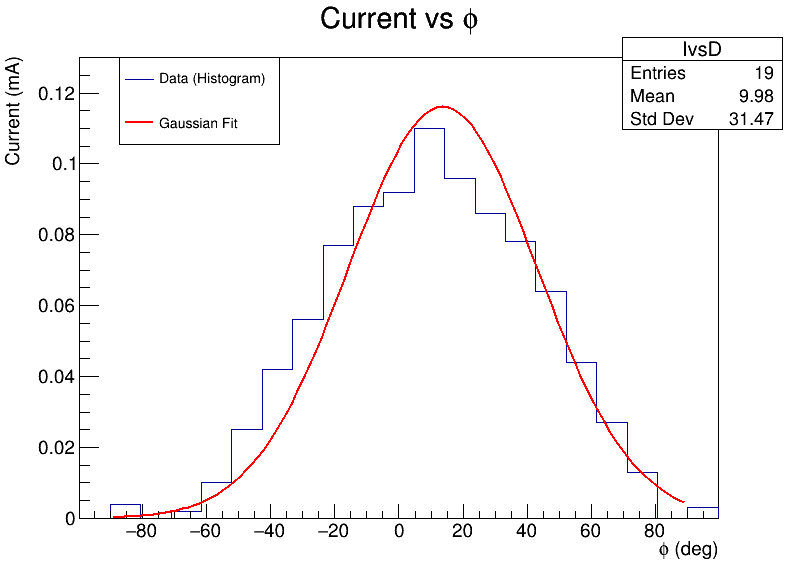
\includegraphics[width=\linewidth]{../plots/I_vs_D.png}
    \caption{Light intensity versus angle between polarizers. The periodic pattern follows Malus's Law with maxima at $0^\circ$ and $180^\circ$, and minima at $90^\circ$ and $270^\circ$.}
    \label{fig:intensity_vs_angle}
\end{figure}

\begin{figure}[H]
    \centering
    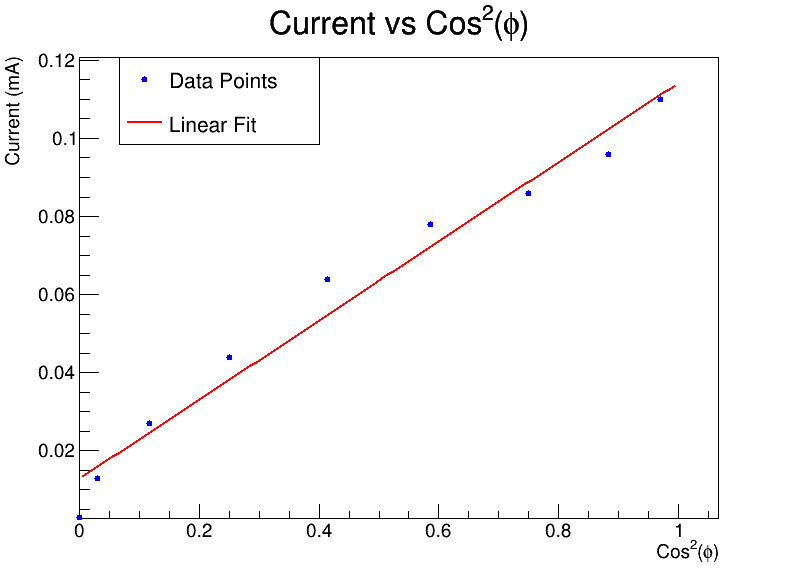
\includegraphics[width=\linewidth]{../plots/I_vs_Cos2Phi.png}
    \caption{Light intensity versus $\cos^2\theta$, showing the linear relationship predicted by Malus's Law.}
    \label{fig:intensity_vs_cos2}
\end{figure}

\section{Part Two: Additional Experiment}

\subsection{Data Tables}
\begin{table}[H]
    \centering
    \caption{Measured current at different angles of the analyzer for the additional experiment.}
    \label{tab:additional_intensity_measurements}
    \pgfplotstabletypeset[
        col sep=comma,
        string type,
        columns={Theta_deg,I_mA_set1,I_mA_set2,I_mA_set3,I_mA_set4},
        columns/Theta_deg/.style={column name=$\theta$ (deg)},
        columns/I_mA_set1/.style={column name=Set 1 (mA)},
        columns/I_mA_set2/.style={column name=Set 2 (mA)},
        columns/I_mA_set3/.style={column name=Set 3 (mA)},
        columns/I_mA_set4/.style={column name=Set 4 (mA)},
        every head row/.style={before row=\toprule,after row=\midrule},
        every last row/.style={after row=\bottomrule},
    ]{../DATA/data_part_2.csv}
\end{table}

\subsection{Graphical Analysis}
The following figures present the relationship between light intensity and polarizer angle for the additional experiment.

\begin{figure}[H]
    \centering
    \includegraphics[width=\linewidth]{../plots/I_vs_D_part2.png}
    \caption{Light intensity versus angle between polarizers for the additional experiment.}
    \label{fig:intensity_vs_angle_part2}
\end{figure}

\begin{figure}[H]
    \centering
    \includegraphics[width=\linewidth]{../plots/I_vs_Cos2Phi_part2.png}
    \caption{Light intensity versus $\cos^2\theta$ for the additional experiment, showing the linear relationship predicted by Malus's Law.}
    \label{fig:intensity_vs_cos2_part2}
\end{figure}

\section{Discussion}

\subsection{Verification of Malus's Law}
The experimental results strongly support Malus's Law:

1. Figure \ref{fig:intensity_vs_angle} shows the characteristic periodic variation in intensity with angle, matching the expected $\cos^2\theta$ dependence.

2. Figure \ref{fig:intensity_vs_cos2} demonstrates the linear relationship between intensity and $\cos^2\theta$, confirming the theoretical prediction.

\subsection{Sources of Error}
Several factors may contribute to experimental uncertainty:
\begin{itemize}
    \item Light detector sensitivity variations
    \item Background light interference
    \item Imperfect polarizer alignment
\end{itemize}

\section{Conclusion}
The experimental results provide strong validation of Malus's Law. The measured intensity variations closely follow the predicted $\cos^2\theta$ relationship, with maximum transmission at aligned polarizers ($0^\circ$, $180^\circ$) and minimum transmission at perpendicular orientations ($90^\circ$, $270^\circ$). These findings have significant implications for applications in optical technologies and material analysis.

\section{Additional Resources}
For detailed information, including the Lab Manual, source code, and related experiments, visit the GitHub repository provided below or scan the QR code in Fig.~\ref{fig:qr_code}.

\begin{figure}[H]
    \centering
    \begin{minipage}{0.15\textwidth}
        \centering
        \qrcode[height=2cm]{https://github.com/ibeuler/LAB-Reports}
    \end{minipage}%
    \begin{minipage}{0.2\textwidth}
        \raggedright
        \caption{Access the GitHub repository for the lab manual, source code, and related experiments: \href{https://github.com/ibeuler/LAB-Reports}{\url{https://github.com/ibeuler/LAB-Reports}}.}
        \label{fig:qr_code}
    \end{minipage}
\end{figure}

\begin{thebibliography}{9}
\bibitem{lab_manual}
    ISTANBUL UNIVERSITY, \textit{Physics Laboratory II Experiment Book: Optics}, Department of Physics, 2024.

\bibitem{github}
    \textit{Source code and additional experiments are available in the GitHub repository.} \url{https://github.com/ibeuler/LAB-Reports}
\end{thebibliography}

\end{document}